\chapter{Linear Algebra}

\section{Fundamental Building Blocks}%
\label{subsec:label}

We will introduce some important subjects to know about deep learning from linear algebra.

A \textbf{scalar} is simply a number. Usually \(x \in \mathbb{R}\) or \(x \in \mathbb{N}\).

A \textbf{vector} is an array of numbers, arranged in order. You can identify each number in the vector by an index.
\begin{equation*}
	\mathbf{x} = \begin{bmatrix} x_1 \\ \vdots \\ x_d \end{bmatrix}
	\quad \text{and} \quad
	\mathbf{x}^T = [x_1, \dots, x_d], \quad \mathbf{x} \in \mathbb{R}^d
\end{equation*}

By $\mathbb{R}^{d}$ it is meant that there are $d$ numbers, all of which real.
We think of vectors as points in space. Each element gives a coordinate along an axis.

A \textbf{matrix} is a 2D array of numbers. Like a vector, this is also identified by indices. However, for matrices there are two, as it has two dimensions.
\begin{equation*}
	\mathbf{A} = \begin{bmatrix} A_{1,1} & A_{1,2} \\ A_{2,1} & A_{2,2} \end{bmatrix}
\end{equation*}
You can also specify entire rows and columns: $A_{i:}$ is the $i$th row, and $A_{:j}$ is the $j$th column. Given a matrix with $m$ rows and $n$ columns called $A$, we say that $A \in \mathbb{R}^{m \times n}$.

A \textbf{tensor} is for when we need an array with more than two axes. An element $(i,j,k)$ of a tensor is denoted by $A_{i,j,k}$. \textbf{An example} of this is an RGB image: This is a tensor of height, width and colour channel. The number of axes is also denoted as \textbf{the rank} of the tensor.

\section{Vectors}%
\label{sec:vectors}

Vectors are often depicted as arrows in Euclidean space. Let us assume we have two vectors, $\mathbf{a}$ and $\mathbf{b}$.
\[
	\mathbf{a} = \begin{pmatrix} 1 \\ 3 \end{pmatrix}
	\quad \text{and} \quad
	\mathbf{b} = \begin{pmatrix} 4 \\ 2 \end{pmatrix}
\]

We can write those vectors as arrows. Seen in Figure~\ref{fig:aandb}, where $\mathbf{a}$ is the red arrow, and $\mathbf{b}$ is blue.
\begin{figure}[ht]
	\centering
	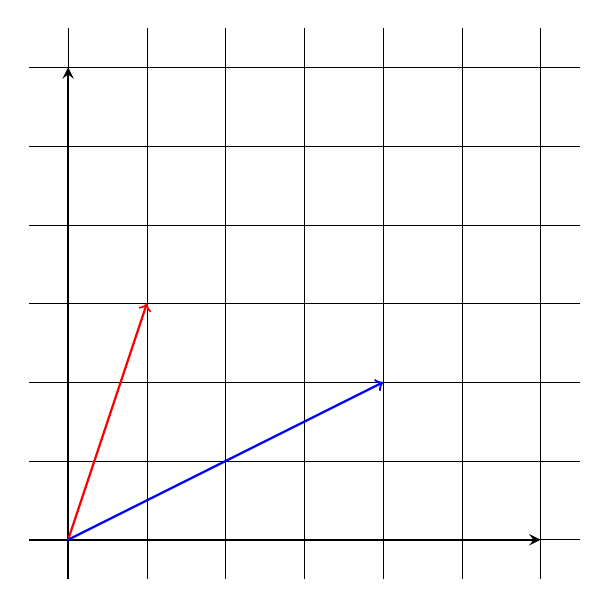
\begin{tikzpicture}
		% Draw axes
		\draw[thick, ->, >=stealth] (-0.5,0) -- (6,0) node[right] {};
		\draw[thick, ->, >=stealth] (0,-0.5) -- (0,6) node[above] {};

		% Draw grid
		\draw[very thin, black] (-0.5,-0.5) grid (6.5,6.5);

		% Draw vectors
		\draw[thick, ->, red] (0,0) -- (1,3);
		\draw[thick, ->, blue] (0,0) -- (4,2);
	\end{tikzpicture}
	\caption{\label{fig:aandb} $\mathbf{a}$ and $\mathbf{b}$}
\end{figure}

We can multiply vectors by a scalar. If we think of it Euclidean, the arrow will \textit{grow} by the size of the scalar. For example:

\[
	\mathbf{a} \cdot 2 = 2 \cdot \begin{pmatrix}
		1 \\
		3
	\end{pmatrix} = \begin{pmatrix}
		2 \cdot 1 \\
		2 \cdot 3
	\end{pmatrix} = \begin{pmatrix}
		2 \\
		6
	\end{pmatrix}
\]

The result can be found in Figure~\ref{fig:scalarmultiplicationtovectors}.
\begin{figure}[ht]
	\centering
	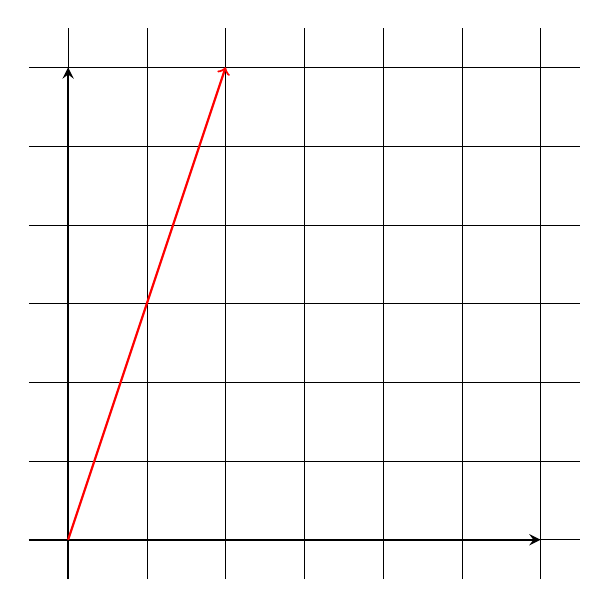
\begin{tikzpicture}
		% Draw axes
		\draw[thick, ->, >=stealth] (-0.5,0) -- (6,0) node[right] {};
		\draw[thick, ->, >=stealth] (0,-0.5) -- (0,6) node[above] {};

		% Draw grid
		\draw[very thin, black] (-0.5,-0.5) grid (6.5,6.5);

		% Draw vectors
		\draw[thick, ->, red] (0,0) -- (2,6);
	\end{tikzpicture}
	\caption{\label{fig:scalarmultiplicationtovectors} $\mathbf{a} \cdot 2$}
\end{figure}

You can also add two vectors together.
\[
	x+ y =
	\begin{pmatrix}
		x_{1}  \\
		\vdots \\
		x_{d}
	\end{pmatrix} + \begin{pmatrix}
		y_{1}  \\
		\vdots \\
		p_{d}
	\end{pmatrix} =
	\begin{pmatrix}
		x_{1} + y_{1} \\
		\vdots        \\
		x_{d} + y_{d}
	\end{pmatrix}
\]

The same goes for subtraction:

\[
	x+ y =
	\begin{pmatrix}
		x_{1}  \\
		\vdots \\
		x_{d}
	\end{pmatrix} - \begin{pmatrix}
		y_{1}  \\
		\vdots \\
		p_{d}
	\end{pmatrix} =
	\begin{pmatrix}
		x_{1} - y_{1} \\
		\vdots        \\
		x_{d} - y_{d}
	\end{pmatrix}
\]

When thinking of these Euclidian, you can think of one vector arrow being added or subtracted from the other, at the tip, such that ones beginning starts at the other's tip.

Another operation is the \textbf{dot product}. This gives us the result of a real number, rather than a vector as was the case before:

\[
	x \cdot y =
	\begin{pmatrix}
		x_{1}  \\
		\vdots \\
		x_{d}
	\end{pmatrix} \cdot \begin{pmatrix}
		y_{1}  \\
		\vdots \\
		p_{d}
	\end{pmatrix} =
	x_{1}y_{1} + x_{2}y_{2} + \cdots + x_{d}y_{d} = \sum_{i=1}^d x_{i}d_{i} = x^{T}y
\]

As the result is a scalar value, this is also called the scalar product or inner product. The dot product obeys many laws that hold for ordinary products of real numbers. Let $a,b,c$ be vectors and \(\lambda\) a scalar. Then:

\begin{enumerate}
	\item $a \cdot b = b \cdot a$
	\item $a \cdot (b + c) = a \cdot b + a \cdot c$
	\item $(\lambda a) \cdot b = \lambda(a \cdot b) = a \cdot (\lambda b)$
	\item \(0 \cdot a = 0\)
\end{enumerate}

The \textbf{length} of the vector is usually calculated as the square root of the summed squares of the entries:

\begin{equation*}
	|x| = \left| \begin{pmatrix}
		x_{1}  \\
		\vdots \\
		x_{d}
	\end{pmatrix} \right|
	=
	\sqrt{x_{1}^{2}+ \cdots + x^{2}_{d}} = \left(  \sum_{i=1}^d x^{2}_{1} \right)^{\frac{1}{2}}
\end{equation*}

This is just a member of a family of \textit{norms}, called $L^{p}$ norms:

\begin{equation*}
	L^{p} = \left(  \sum_{i} |x_{i}|^{p} \right)^{\frac{1}{p}}
\end{equation*}

$L^{2}$ norm is the most commonly used, and if nothing else is stated, this is the norm used. Also called the Euclidian norm. The max norm is $L^{\infty} = \left| \left| x \right| \right|_{\infty} = \max \left| x_{i} \right|$.

The dot product of two vectors can be written in terms of their $L^{2}$ norms and an angle \(\theta\) between them:

\[
	x \cdot y = |x| |y| \cdot \cos \theta
\]

Example with the previous two vectors we used, $\mathbf{a}$ and $\mathbf{b}$:
\[
	\theta = \cos^{-1} \left( \frac{\mathbf{a}\mathbf{b}}{|a| \cdot |b|} \right)
\]
\[
	= \cos^{-1} \left( \frac{10}{\sqrt{10} \cdot \sqrt{20}} \right) = 45^{\circ}
\]

\subsection{Matrices}%
\label{subsec:matrices}

The \textbf{order} of the matrix represents the number of rows and number of columns. For a matrix with 3 columns and 3 rows, the order would be $3 \times 3$. This is an example of a \textbf{square matrix}, which is a matrix whose column and row size is equal. There are also a few special matrices:
\begin{itemize}
	\item \textit{Row Matrix}: If a matrix only has one row: also a transposed vector
	\item \textit{Column Matrix}: If a matrix only has one column: a vector
	\item \textit{$1 \times 1$ Matrix}: A Scalar
\end{itemize}

You add two matrices by adding each of their elements:
\[
	\begin{pmatrix} a & b \\ c & d \end{pmatrix}
	+ \begin{pmatrix} e & f \\ g & h \end{pmatrix}
	= \begin{pmatrix} a + e & b + f \\ c + g & d + h \end{pmatrix}
\]
It is necessary for the matrices to have the same order (or dimensionality).

You can also multiply a matrix by a scalar \(\lambda\):
\[
	\lambda \cdot \begin{pmatrix} a & b \\ c & d \end{pmatrix}
	= \begin{pmatrix} \lambda \cdot a & \lambda \cdot b \\ \lambda \cdot c & \lambda \cdot d \end{pmatrix}
\]

You can also multiply two matrices. To do this, you perform the dot product between rows of the first matrix and columns of the second matrix:
\[
	\mathbf{A \cdot B = C}
\]
\[
	c_{i,j} = \sum_k a_{ik}b_{kj}
\]

Thus two matrices can only be multiplied if the number of columns in the first matrix is equal to the number of rows in the second matrix. I.e., if \textbf{A} is of order $m \times n$ and \textbf{B} is of order $r \times s$, then $A \cdot B$ is possible if $r = n$. The resulting matrix will be of order $m \times s$.

There are some properties to the matrix product:
\begin{itemize}
	\item Distributivity over addition: \(A(B+C) = AB+AC\)
	\item Associativity: \(A(BC) = (AB)C\)
	\item \textbf{Not commutative}.
	      \begin{itemize}
		      \item However, is between two vectors: $x^{T}y = y^{T}x$
	      \end{itemize}
	\item Transpose of a matrix product has a simple form: $(AB)^{T} = B^{T}A^{T}$
\end{itemize}

The norm of a matrix is analogous to $L^{2}$ form of a vector:
\[
	||A|| = \left( \sum_{i,j} A_{i,j}^{2} \right)^{\frac{1}{2}}
\]

\subsection{Square Matrices}%
\label{subsec:label}

There are some operations special to square matrices, which are not defined for arbitrary matrices.

An \textit{identity matrix} (or unit matrix) of size $d$ is a square matrix of order $d \times d$ where all the diagonal elements are '1' and all other elements are '0'. It is denoted by $I$:
\[
	I_1 = (1) \quad
	I_2 = \begin{pmatrix} 1 & 0 \\ 0 & 1 \end{pmatrix} \quad
	I_3 = \begin{pmatrix} 1 & 0 & 0 \\ 0 & 1 & 0 \\ 0 & 0 & 1 \end{pmatrix}
\]

For a square matrix $A$, we have an important property:
\[
	A \cdot I = I \cdot A = A
\]

The \textbf{inverse} of a matrix is defined as being the matrix whose product with the original matrix produces an identity matrix:

\[
	AA^{-1} = A^{-1}A = I
\]

However, not all square matrices have inverses. Those who do are called \textit{invertible} or are said to be \textit{nonsingular matrices}. A square matrix which does not have an inverse is called noninvertible or singular matrix. A square matrix is singular if and only if its determinant is 0.

We will now look at \textit{determinants}. The determinant of a square matrix $det(A)$ is a mapping to a scalar. It is equal to the product of all eigenvalues of the matrix. It measures how much multiplication by the matrix expands or contracts space.

\noindent
\textbf{For a 1x1 matrix:}
\[
	\det(a_{11}) = a_{11}
\]

\noindent
\textbf{For a 2x2 matrix:}
\[
	\begin{vmatrix}
		a_{11} & a_{12} \\
		a_{21} & a_{22}
	\end{vmatrix}
	= a_{11}a_{22} - a_{12}a_{21}
\]

\noindent
\textbf{For a 3x3 matrix:}
\[
	\begin{vmatrix}
		a_{11} & a_{12} & a_{13} \\
		a_{21} & a_{22} & a_{23} \\
		a_{31} & a_{32} & a_{33}
	\end{vmatrix}
	= a_{11}(a_{22}a_{33} - a_{23}a_{32}) - a_{12}(a_{21}a_{33} - a_{23}a_{31}) + a_{13}(a_{21}a_{32} - a_{22}a_{31})
\]

\subsection{Special vectors and matrices}%
\label{subsec:label}

A \textit{unit vector} is a vector with unit norm $||x||_{2}=1$.

A vector $x$ and vector $y$ are said to be orthogonal to each other if $x^{T}y=0$. Meaning vectors are at 90 degrees to each other.

An \textit{orthogonal matrix} is a square matrix whose columns and rows are orthogonal unit vectors $A^{-1} = A^{T}$

A \textit{diagonal matrix} is a matrix with mostly zeroes, except for the diagonal, which contains non-zero entries. $diag(\mathbf{v})$ is a square diagonal matrix with diagonal elements given by entries of vector $\mathbf{v}$. Multiplying $diag(v)$ by vector $x$ only needs to scale each element $x_{i}$ by $v_{i}$.

A \texttt{symmetric matrix} is a matrix which is equal to its transpose:
\[
	A = A^{T}
\]






%%% Local Variables:
%%% mode: latex
%%% TeX-engine: luatex
%%% TeX-command-extra-options: "-shell-escape"
%%% TeX-master: "main"
%%% End:
